\documentclass[10pt]{beamer}
\usepackage[slovene]{babel}
\usepackage[utf8]{inputenc}
\usepackage[T1]{fontenc}
\usepackage{lmodern}
\usepackage{mathptmx}
\usepackage{helvet}
\usepackage{courier}
\usepackage{hyperref}
\usepackage{wrapfig}
\usepackage{tikz}
\usepackage{tcolorbox}

\usetheme{CambridgeUS}

\begin{document}

\title[Kazalniki ekonomske neenakosti]{Kazalniki ekonomske neenakosti}
\author{Eva Deželak, Žan Jarc, Veronika Sovdat in Ines Šilc}
\institute [FMF]{ Fakulteta za matematiko in fiziko}

\begin{frame}
	\titlepage
\end {frame}

\begin{frame}
Vsebina predavanja:
	\begin{itemize}
		\item Definicije osnovnih pojmov
		\item Tekma med izobraževanjem in tehnologijo
		\item Posamezni kazalniki neenakosti
			\begin{itemize}
				\item Ginijev koeficient
				\item Lorenzova krivulja
				\item Palmovo razmerje
				\item Kazalnika revščine
			\end{itemize}
		\item Ekonomska neenakost in demokracija
	\end{itemize}
\end {frame}

\begin{frame}
\frametitle{Definicije osnovnih pojmov}
\begin{itemize}
\item \textbf{Državni dohodek} je vsota vseh dohodkov, ki so na voljo prebivalcem neke države v danem letu, ne glede na klasifikacijo dohodkov.
$$
\textbf{Državni dohodek} = \textbf{BDP} - \textbf{cena kapitala} + \textbf{neto dobiček iz tujine}
$$
\item \textbf{Državno premoženje} je vsota privatnega in javnega premoženja.
$$
\textbf{Državno premoženje}~=~\textit{domači kapital}~+~\textit{neto tuji kapital}
$$
\item Neenakost v odnosu do dela in kapitala. Plače so ena oblika dohodka iz dela, dohodek iz kapitala pa predstavlja vse prihodke, ki jih ima lahko nek posameznik od kapitala, to so lahko na primer najemnine, dividende, obresti\dots
\end{itemize}
\end{frame}

\begin{frame}
\frametitle{Tekma med izobraževanjem in tehnologijo}
\begin{itemize}
\item Teorija ima dve predpostavki:
\begin{enumerate}
\item Plača delavca je enaka njegovi \textbf{mejni produktivnosti}.
\item Produktivnost delavca je odvisna od njegovih spretnosti in strokovnega znanja ter \textbf{ponudbi} teh spretnosti v dani družbi.
\end{enumerate}


\item Teorija o tekmi med izobraževanjem temelji predvsem na ponudbi in povpraševanju strokovnega znanja v neki državi. 
\item Tehnološki napredek je odvisen od hitrosti inovacij in hitrosti implementacije teh inovacij. Ponavadi dvigne povpraševanje za nova strokovna znanja in ustvari nova delovna mesta.


\item Pomanjkljivosti:
\begin{enumerate}
\item Plača $\neq$ mejna produktivnost
\item Ne razloži gromozanskih razlik med plačami direktorjev in delavci podjetja.
\end{enumerate}
\end{itemize}
\end{frame}

\begin{frame}
\frametitle{Ginijev koeficient}

\begin{columns}[T]
    \begin{column}{.5\textwidth}
     \begin{block}{}
\begin{itemize}
\item Italijanski statistik Corrado Gini (1884 - 1965).
\item Število 0 predstavlja popolno enakost, število 1 pa popolno neenakost. 
\item PRIMER: 10 \% svetovnega prebivalstva si lasti 87,7 \% celotnega svetovnega bogastva.
\end{itemize}
    \end{block}{}
    \end{column}
    \begin{column}{.5\textwidth}
    \begin{block}{Corrado Gini}
    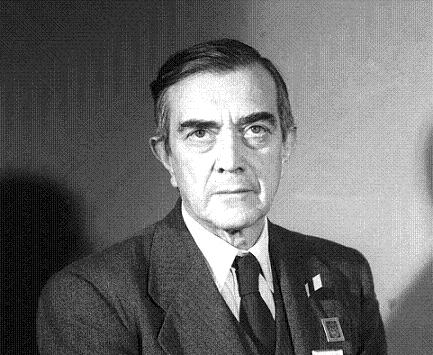
\includegraphics[width=0.9\textwidth]{./slike/corrado-gini.jpg}
    \end{block}{}
    \end{column}
  \end{columns}
\end{frame}

\begin{frame}
\frametitle{Lorenzova krivulja}
\begin{itemize}
\item Populacija velikosti N, količina Q. 
\item Z L(p) označimo del količine Q, ki si jo lasti del populacije v prvem p-tem deležu.
\item Graf funkcije L(p) imenujemo \textbf{Lorenzova krivulja}.
\item Popolna enakomerna porazdelitev premoženja: L(p) = p.
$$\Rightarrow 0 \leq L(p) \leq p$$
\begin{tcolorbox}[colback=black!5,colframe=red!40!black,title=Ginijev koeficient]
$$G := 2 \cdot \int_{0}^{1} (p - L(p)) dp$$
\end{tcolorbox}
\item Ker je  $0 \leq \int_{0}^{1} (p - L(p)) dp \leq \int_{0}^{1} p dp = \frac{1}{2}$, je $G \in [0, 1].$
\end{itemize}
\end{frame}

\begin{frame}
\frametitle{Ekonomska neenakost doma in po svetu}
\begin{figure}
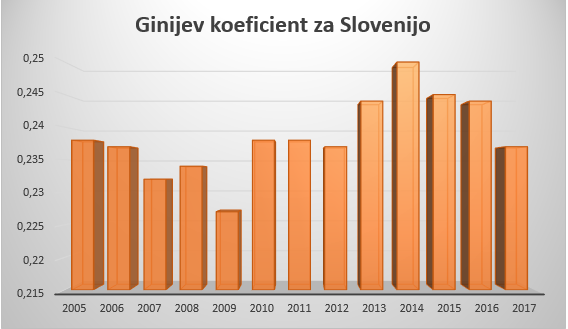
\includegraphics[width= \linewidth]{./slike/gini-slo.PNG}
\end{figure}
\end{frame}

\begin{frame}
\frametitle{Ekonomska neenakost doma in po svetu}
\begin{figure}
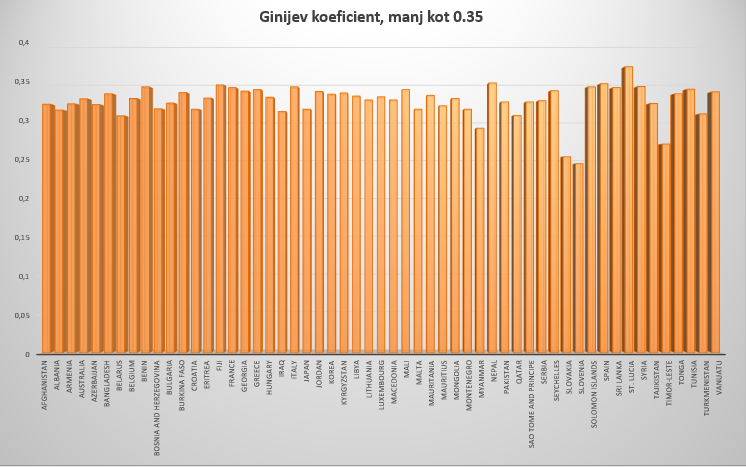
\includegraphics[height=.3 \textwidth, width = .7\linewidth]{./slike/gini-manj-07.PNG}
\hspace{0.3\textwidth}
\hfill
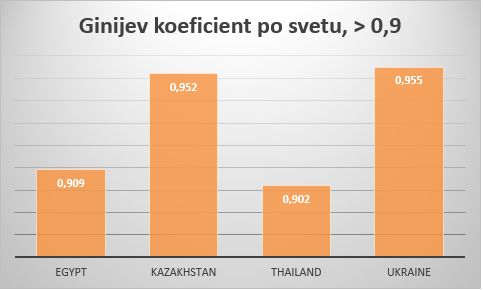
\includegraphics[height=.3 \textwidth, width = .6\linewidth]{./slike/gini-vec-09.PNG}
\end{figure}
\end{frame}





\begin{frame}
\frametitle{Palmovo razmerje}
\begin{itemize}
\item Kazalnik ekonomske neenakosti:

\begin{itemize}
\item $b := \textrm{delež dohodka, ki pripada 10\% prebivalstva z najvišjim dohodkom},$
\item $r := \textrm{delež dohodka, ki pripada 40\% prebivalstva z najnižjim dohodkom},$
\end{itemize}
$$
\textrm{Palmovo razmerje} := \frac{b}{r}.
$$

\item Lastnosti:
\begin{itemize}
\item osredotoči se na krajišča (na najrevnejše in najbogatejše prebivalstvo),
\item odzivno na visoko neenakost (Ginijev koeficijent opazi samo nizko neenakost),
\item preprost izračun.
\end{itemize}
\end{itemize}
\end{frame}

\begin{frame}
\frametitle{Graf: Palmovo razmerje in Ginijev koeficient}
\begin{figure}
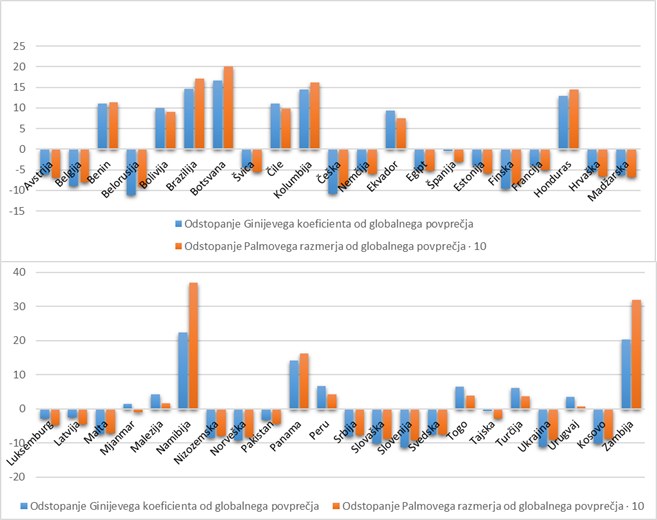
\includegraphics[scale = 0.6]{./slike/gini_palma.png}
\end{figure}

\end{frame}



\begin{frame}
\frametitle{Indikatorji revščine in posledično kazatelji neenakosti}
\begin{itemize}
\item \textbf{Stopnja tveganja revščine} - procent ljudi, ki živijo pod pragom revščine.

\item \textbf{Indeks revščine (PGI)}:
\begin{itemize}
\item $N := \textrm{število prebivalcev}$,
\item $q := \textrm{število prebivalcev, ki živijo pod pragom revščine}$,
\item $z := \textrm{prag revščine}$,
\item $q_i := \textrm{dohodek revnega prebivalca i}$,
\end{itemize}
$$
PGI = \frac{1}{N} \cdot \sum_{i=1}^q (\frac{z-q_i}{z}).
$$
\end{itemize}
\end{frame}


\begin{frame}
\frametitle{Graf: Stopnja tveganja revščine in Ginijev koeficient}
\begin{figure}
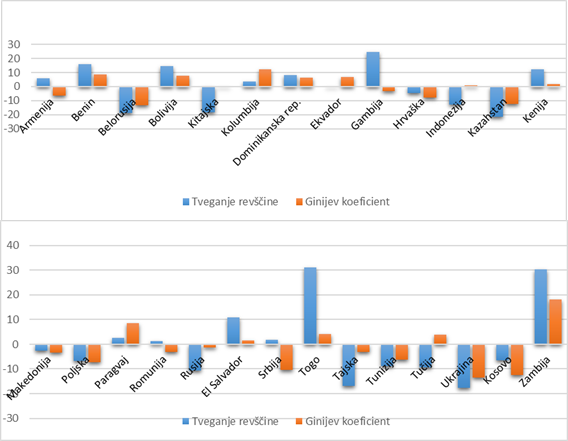
\includegraphics[scale = 0.71]{./slike/gini_revscina3.png}
\end{figure}

\end{frame}

\begin{frame}
\frametitle{Ekonomska neenakost in demokracija}
\begin{itemize}
\item \textbf{Demokracija} je oblika vladavine, v kateri oblast, oziroma pravica vladati, izvira iz ljudstva.
\item Ogledali si bomo kako ekonomska neenakost vpliva na osrednje lastnosti demokracij.
\item Tri različne teorije, ki vsaka različno razlaga povezavo med ekonomsko neenakostjo in politično vključenost prebivalcev v demokratičnih državah:
	\begin{itemize}
	\item \textbf{teorija relativne moči},
	\item \textbf{konfliktna teorija},
	\item \textbf{teorija sredstev}.
	\end{itemize}
\end{itemize}
\end{frame}

\begin{frame}
\frametitle{Teorija relativne moči}
\begin{itemize}
\item Ekonomska neenakost naj bi imela negativen učinek na politilčno vključenost celotnega prebivalstva.
\item Učinek naj bi bil še večji pri revnejših posameznikih.
\item To zagovarja s predpostavka, da denar lahko vpliva na posameznike.
\item Bogatejši posamezniki lahko s svojim premoženjem premagujejo konflikte, ki nastajajo v državi.
\item Manj premožni dobijo občutek nezmožnosti premagovanja ovir.
\item Premožni so politično vključeni le še zaradi zavarovanja svojega statusa in zaradi konfliktov med sami sebe.
\end{itemize}
\end{frame}

\begin{frame}
\frametitle{Konfliktna teorija}
\begin{itemize}
\item Ravno nasprotno kot teorija relativne moči.
\item Neenakost naj bi spodbudila politično vključenost posameznikov.
\item Višje stopnje neenakosti naj bi sprožile razkorak v državi in spodbudile debate.
\item Revnejši v svoji politični angažiranost vidijo pot do izboljšanja svojih okoliščin.
\item Z redestribucijo se ne strinjajo bogatejši.
\item Večja kot bo neenakost, večji bo razkorak v pogledih revnih in bogatih.
\end{itemize}
\end{frame}

\begin{frame}
\frametitle{Teorija sredstev}
\begin{itemize}
\item Teorija sredstev predpostavlja, da ima lahko ekonomska neenakost pozitivni ali negativni učinek na politično vključenost posameznikov.
\item Angažiranost je odvisna od posameznikovih sredstev.
\item Predpostavlja, da vsaka angažiranost potrebuje sredstva (denar, čas, sposobnost).
\item Posameznik naj bi gledal na politično vključenost kot na vsako drugo dobrino.
\item Pri večji neenakosti bi morala biti vključenost revnejših nižja, bogatejših pa višja.
\end{itemize}
\end{frame}

\begin{frame}
\frametitle{Economic Inequality and Democratic Politcal Engagement, Frederick Solt, 2008}
\begin{itemize}
\item V tem članku je želel avtor analizirati kako ekonomska neenakost vpliva na politično vključenost v premožnejših demokratskih državah.
\item Politično vključenost posameznikov je razdelil na tri dele:
	\begin{itemize}
	\item \textbf{politični interes},
	\item \textbf{politična diskusija},
	\item \textbf{volitvena udeležba}.
	\end{itemize}
\item S podatki je ovrgel konfliktno teorijo in teorijo sredstev.
\end{itemize}
\end{frame}







\begin{frame}
\frametitle{Viri}
	\begin{itemize}
		\item
			\label{Pickety}
			T.~Pickety, \emph{Capital in the twenty-first century}, The Belknap Press of 						Harvard University Press, London, 2014.

		\item 
			\label{Razdelitev premoženja}
			\emph{Distribution of wealth}, v: Wikipedia, The Free Encyclopedia, [ogled 							20.~4.~2019], dostopno na \url{https://en.wikipedia.org/w/index.php?								title=Distribution_of_wealth&oldid=854198883}.

		\item 
			\label{Metrike ekonomske neenakosti}
			\emph{Income inequality metrics}, v: Wikipedia, The Free Encyclopedia, [ogled 					20.~4.~2019], dostopno na \url{https://en.wikipedia.org/w/index.php?								title=Income_inequality_metrics&oldid=853906711}.

\item
\emph{Ginijev koeficient}, Janja Trogar, [ogled 3.~5.~2019], dostopno na \url{https://repozitorij.uni-lj.si/IzpisGradiva.php?id=97164}.

\item
\emph{Statistični urad RS}, Neenakost porazdelitve dohodka - Ginijev količnik (\%), Slovenija, letno, [ogled 4.~5.~2019], dostopno na \url{https://pxweb.stat.si/pxweb/Dialog/varval.asp?ma=0867312S&ti=&path=../Database/Dem_soc/08_zivljenjska_raven/08_silc_kazalniki_revsc/15_08673_porazdel_dohodka/&lang=2}.
\item
			F.~Solt, \emph{Economic Inequality and Democratic Politcal Engagement}, American Journal of Political Science, Southern Illinois University, 2008.
\end{itemize}
\end {frame}










\end{document}